\section{Exercises}

\paragraph{Exercise 2.1}
\textit{In the comparison in fig~2.1, which method will perform best in the long run in terms of cumulative reward, and cumulative probability of selecting the best action?}

Because of the law of large numbers, in the long run we have $Q_t(a) \approx q(a)$ for $\epsilon$-greedy methods, since each actions will have been sampled a very large number of times.
This is of course not true for the greedy method which correctly sample only one action, the one it always choses.
For $\epsilon$-greedy method, in the long run we select the action $A^* = \argmax_a q(a)$ $(1 - \epsilon)$ of the time and a random action $\epsilon$ of the time.
There doesn't seem to be any exact function that gives the expectation of the maximum of $n$ iid normal variables, I could only find inequalities for large $n$...
I computed the value for $n = 10$ using 1 million series of 10 iid normal variables, and got a value of $\approx 1.54$
The average reward when selecting action $A^*$ is $\mathbb{E}[q(A^*)] \approx 1.54$.
Meanwhile, let $Z$ be the reward when selection a random action, and $Y \sim \mathcal{N}(0,1)$ the noise term added to $q(a)$ when computing the reward.
We have:
\begin{align*}
\mathbb{E}[Z] &= \mathbb{E}[\mathbb{E}[q(a)] + Y] \\
              &= \mathbb{E}[q(a)] + \mathbb{E}[Y] \\
              &= 0
\end{align*}
since both random variables $q(a)$ and $Y$ follow a standard normal distribution.
All in all, for $\epsilon$-greedy method, the average expected reward is:
\begin{align*}
\mathbb{E}[\bar{R}] &= \epsilon \mathbb{E}[Z] + (1 - \epsilon) \mathbb{E}[q(A^*)] \\
                    &\approx (1 - \epsilon) \times 1.54 \\
\end{align*}
Which means 1.39 for $\epsilon = 0.1$ and 1.52 for $\epsilon = 0.01$.

For the true greedy method, the first action $A^\dagger$ for which the reward gets over 0 gets chosen everytime (at first approximation).
Thus we need to find $\mathbb{E}[q(A^\dagger)] = \mathbb{E}[q(a)| q(a) + Y > 0]$.
I could not manage to find a seemingly correct formula unfortunately (but this one should not be too hard for a statistician), so I once again computed an estimate for this number for $n = 10$, and came up with $\mathbb{E}[q(A^\dagger)] \approx 0.56$.
This looks a bit weird since in fig~2.1 the average reward of the greedy method is around $1$.

For $\epsilon$-greedy method, the probability of selecting the best action when we decided to chose a random action is obviously $\frac{1}{n}$.
As for when we decide to chose the action with the highest estimated value, I get stuck.
We need to find, given $(Y, Z) \sim \mathcal{N}(0,1)^2$, the probability $Pr\{q(a) + Y > q(A^*) + Z\}$.
That honestly seems daunting to me and I would not even know where to begin anyway...
Graphically, the curve seems to plateau at around 80\% for $\epsilon = 0.1$, and should be plateauing over this value for $\epsilon = 0.01$.
Same for the greedy method, which seems to plateau at around 35\%.

\paragraph{Exercise 2.2}
\textit{Give pseudocode for a complete algorithm for the $n$-armed bandit problem. Use greedy action selection and incremental computation of action values with $\alpha = \frac{1}{k}$ step-size parameter. Assume a function $\mathit{bandit}(a)$ that takes an action and returns a reward. Use arrays and variables; do not subscript anything by the time index $t$. Indicate how the action values are initialized and updates after each reward. Indicate how the step-size parameters are set for each action as a function of how many times it has been tried.}

\begin{enumerate}
\item Initialization \\
$Q(a) \leftarrow 0$ for all $a \in \mathcal{A}$ \\
$k(a) \leftarrow 1$ for all $a \in \mathcal{A}$

\item Action selection and value update \\
Repeat \\
\-\hspace{2em} $A \leftarrow \argmax_a Q(a)$ (resolve ties randomly) \\
\-\hspace{2em} $R \leftarrow \mathit{bandit}(A)$ \\
\-\hspace{2em} $Q(A) \leftarrow Q(A) + \frac{1}{k} (R - Q(A))$ \\
\-\hspace{2em} $k(A) \leftarrow k(A) + 1$ \\
until end of epoch
\end{enumerate}

\paragraph{Exercise 2.3}
\textit{If the step-size parameters, $\alpha_k$, are not constant, then the estimate $Q_k$ is a weighted average of previously received rewards with a weighting different from that given by (2.6). What is the weighting on each prior reward for the general case, analogous to (2.6), in terms of $\alpha_k$?}

\begin{align*}
Q_{k+1} &= Q_k + \alpha_k (R_k - Q_k) \\
        &= \alpha_k R_k + (1 - \alpha_k) Q_k \\
        &= \alpha_k R_k + (1 - \alpha_k) [\alpha_{k-1} R_{k-1} + (1 - \alpha_{k-1}) Q_{k-1}] \\
        &= \alpha_k R_k + \alpha_{k-1} (1 - \alpha_k) R_{k-1} + (1 - \alpha_{k}) (1 - \alpha_{k-1}) Q_{k-1} \\
        &= Q_1 \prod_{i=1}^k (1 - \alpha_i)  + \sum_{i=1}^k \left( \alpha_i R_i \prod_{j=i+1}^{k} (1 - \alpha_j)  \right) \\
\end{align*}

The weights are then $\prod_{i=1}^k (1 - \alpha_i)$ for $Q_1$ and $\alpha_i R_i \prod_{j=i+1}^{k} (1 - \alpha_j)$ for $R_i$.

\paragraph{Exercise 2.4 (programming experiment)}
\textit{Design and conduct an experiment to demonstrate the difficulties that sample-average methods have for nonstationary problems. Use a modified version of the 10-armed testbed in which all the q(a) start out equal and then take independent random walks. Prepare plots like Figure 2.1 for an action-value method using sample averages, incrementally computed by $\alpha = \frac{1}{k}$, and another action-value method using a constant step-size parameter, $\alpha = 0.1$. Use $\epsilon = 0.1$ and, if necessary, runs longer than 1000 plays.}

See file \textit{exercise\_2\_4.py} for the Python code.
The code is composed with 3 classes (2 for bandit problem definition, Bandit and DriftBandit, and 1 for a general action-value method, EpsGreedyLearner) and 2 functions (run\_drift and experiments) to conduct the experiment.

\begin{figure}[!htb]
\centering
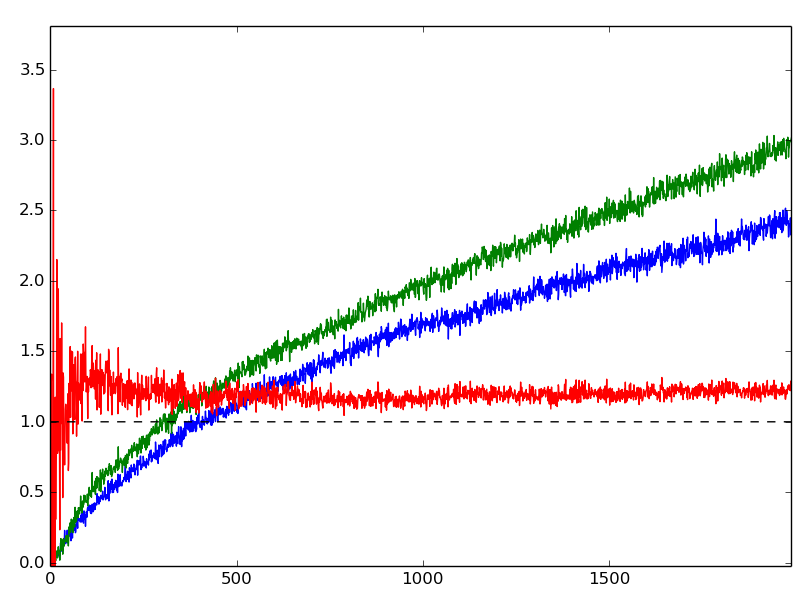
\includegraphics[width=0.47\columnwidth]{chap1_bandits/plot_rewards.png}
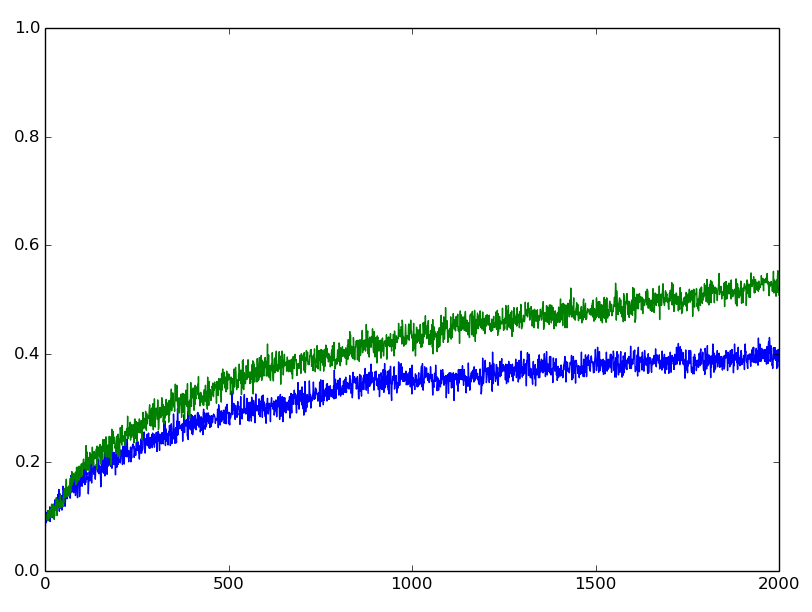
\includegraphics[width=0.47\columnwidth]{chap1_bandits/plot_bestaction.png}
\caption{\label{chap1_fig_ex24}
Left: average rewards (blue: $\alpha = \frac{1}{k}$, green: $\alpha = 0.1$, red: green/blue).
Right: probability of selecting the best action (blue: $\alpha = \frac{1}{k}$, green: $\alpha = 0.1$).
}
\end{figure}

Figure~\ref{chap1_fig_ex24}.left shows that a fixed step-size consistently outperforms the "average" step-size.
Figure~\ref{chap1_fig_ex24}.right clearly shows the difficulty of the action-value method to track a non-stationnary problem.
Indeed, the Figure 2.1 in the original manuscript reports probabilities of selecting the best action to be around 80\% in the long-run for $\epsilon = 0.1$.
For the same $\epsilon$ value, this method only reports probabilities of 50-60\% -- although this number could still increase with a higher number of time steps.
